\section{Конструкторская часть}

В этой части будут приведены требования к программе и схемы алгоритмов нахождения расстояний Левенштейна и Дамерау --- Левенштейна.

\subsection{Требования к программному обеспечению}

Программа должна поддерживать два режима работы:
\begin{enumerate}
    \item ручной ввод;
    \item массированный замер времени.
\end{enumerate}

В режиме ручного ввода пользователь должен иметь возможность
\begin{itemize}
    \item ввести два слова через пробел с клавиатуры;
    \item использовать символы в кодировке \texttt{Unicode};
    \item ввести слова размером до $25\,000$ символов в кодировке \texttt{Unicode}.
\end{itemize}

В режиме ручного ввода программа должна
\begin{itemize}
    \item запустить каждую из реализаций четырёх алгоритмов (итерационного алгоритма нахождения расстояния Левенштейна, итерационного алгоритма нахождения расстояния Дамерау --- Левенштейна, рекурсивного алгоритма нахождения расстояния Дамерау --- Левенштейна, рекурсивного с кешированием алгоритма нахождения расстояния Дамерау --- Левенштейна);
    \item вывести заполненные матрицы расстояний для итерационных алгоритмов нахождения расстояний Левенштейна и Дамерау --- Левенштейна;
    \item вывести последовательность редакторских операций, которая привела к нахождению расстояний Левенштейна и Дамерау --- Левенштейна, для итерационных алгоритмов нахождения расстояний Левенштейна и Дамерау --- Левенштейна;
    \item вывести результат работы каждого алгоритма с названием этого алгоритма.
\end{itemize}

В режиме массированного замера времени пользователь должен иметь возможность
\begin{itemize}
    \item ввести начальную длину строк, конечную длину строк, шаг изменения длин строк, которые будут использоваться в замерах времени;
    \item ввести количество замеров времени, которое требуется произвести для каждой длины строк (в результате будет выдано среднее значение по каждой длине);
    \item посмотреть графики, построенные на основе данных из последнего замера времени.
\end{itemize}

В режиме массированного замера времени программа должна
\begin{itemize}
    \item на основе данных о длинах строк, полученных от пользователя, сгенерировать строки указанных длин из фиксированного набора символов в кодировке \texttt{Unicode}; конкретный символ строки должен выбираться в результате генерации псевдослучайного целого числа по модулю количества символов в фиксированном наборе --- полученное число есть индекс символа в наборе;
    \item каждую пару сгенерированных строк подать на вход всем алгоритмам, время работы реализаций которых требуется измерить;
    \item произвести замеры времени работы для каждой реализации алгоритмов без учёта времени на создание и инициализацию матрицы в тех алгоритмах, где матрица используется;
    \item записать данные о каждом замере времени в файл;
    \item на основе данных из файла построить четыре графика (по графику на каждый алгоритм), где значения по оси $Ox$ --- длины строк, значения по оси $Oy$ --- время работы реализации алгоритма в наносекундах, и вывести результат пользователю.
\end{itemize}

\newpage

\subsection{Разработка алгоритмов}

На вход алгоритмам подаются строки $S1$, $S2$ и их длины $L1$, $L2$ соответственно.

На рисунке \ref{fig:lifm} представлена схема алгоритма нахождения расстояния Левенштейна.
На рисунках \ref{fig:dlifm} -- \ref{fig:dlrwch} представлены схемы алгоритмов нахождения расстояния Дамерау --- Левенштейна.

\begin{figure}[h]
	\centering
	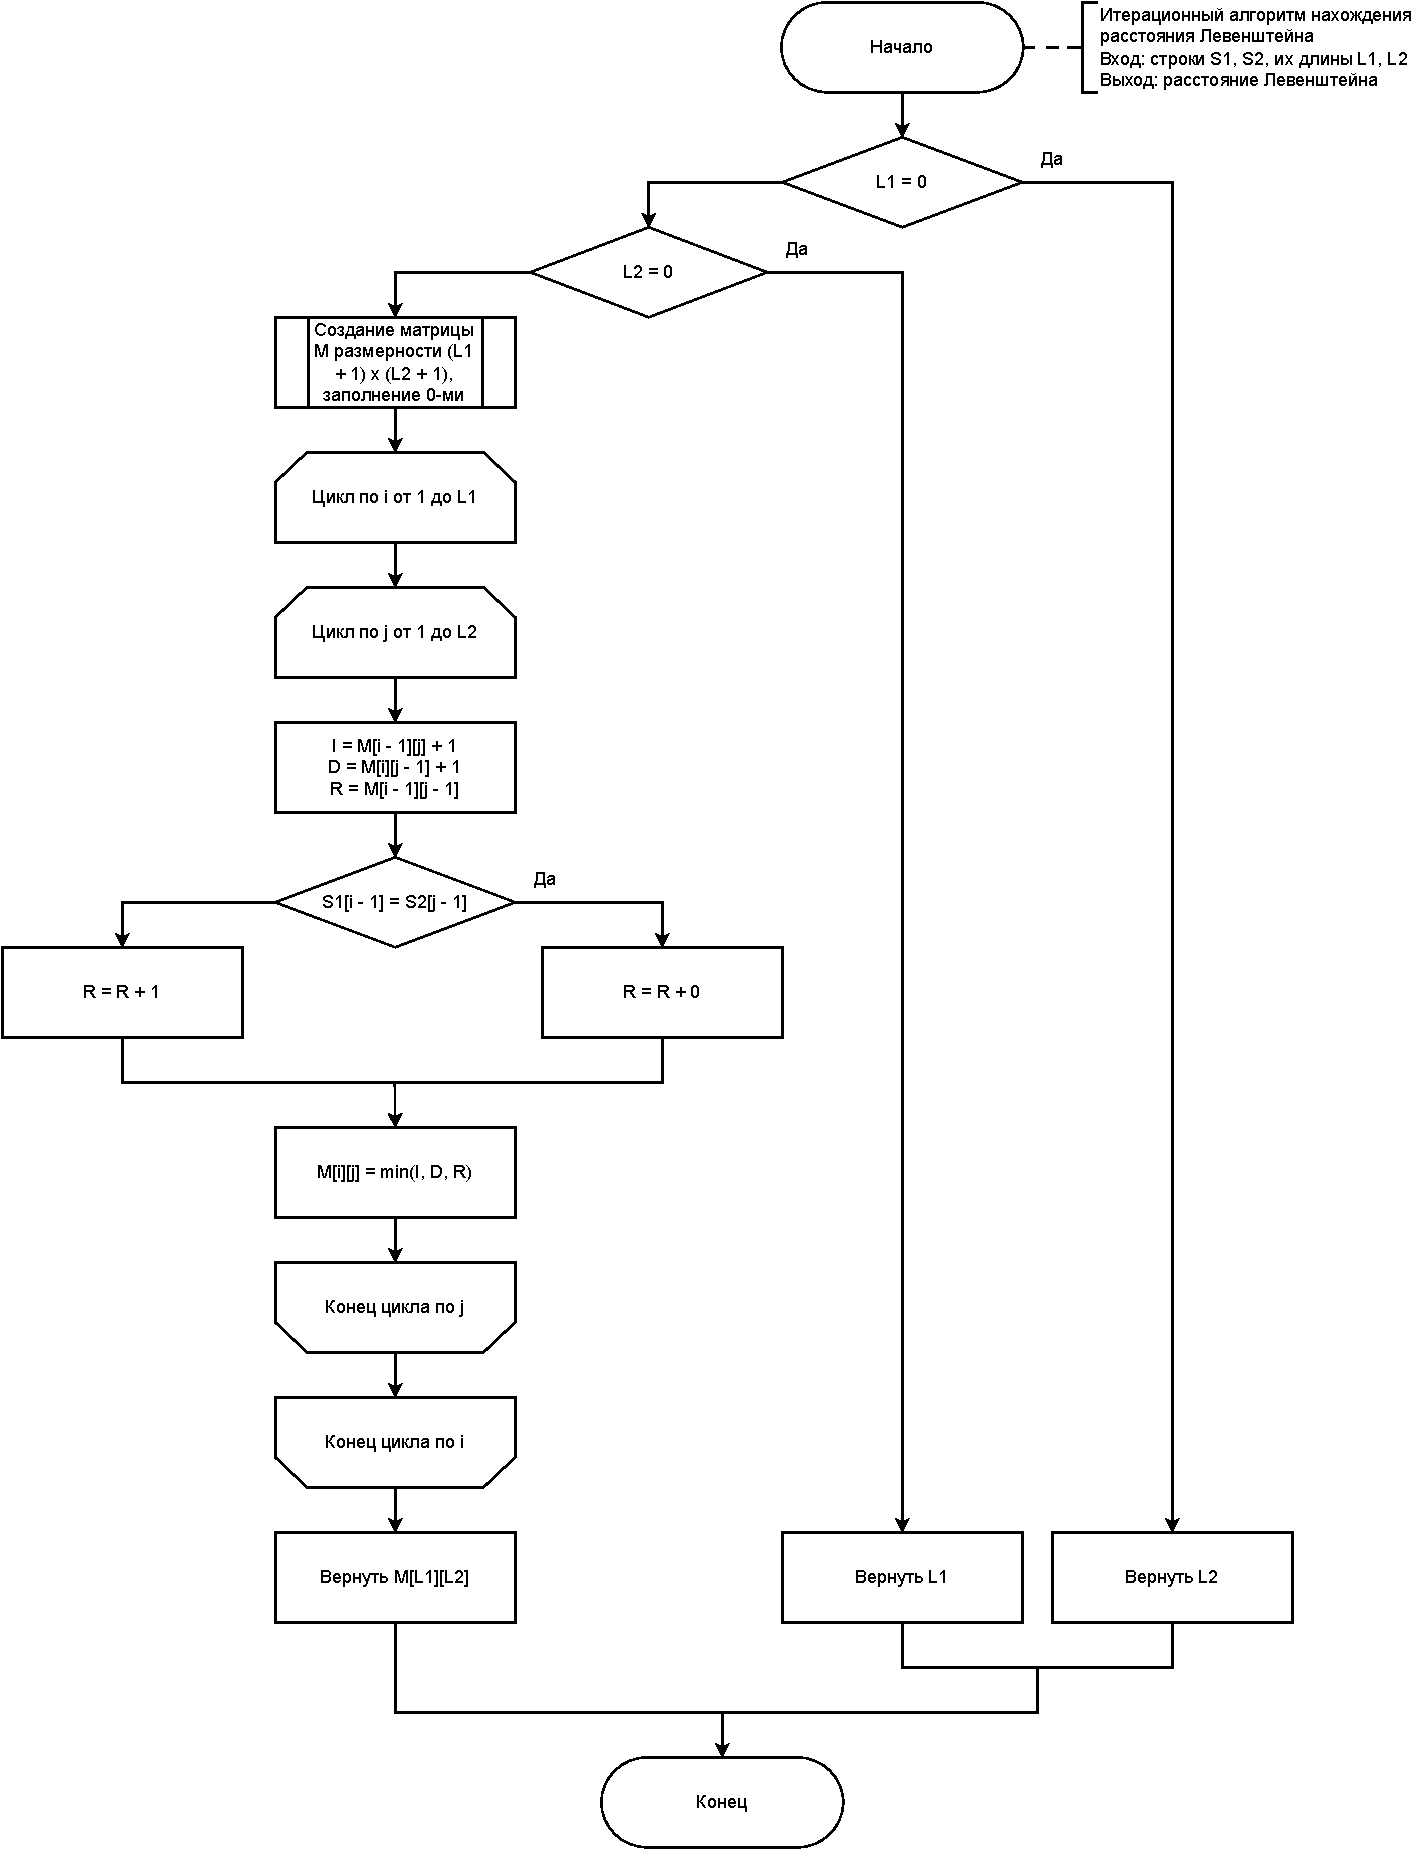
\includegraphics[scale=0.5]{img/lev_ifm.pdf}
	\caption{Итерационный алгоритм нахождения расстояния Левенштейна}
	\label{fig:lifm}
\end{figure}

\begin{figure}[h]
	\centering
	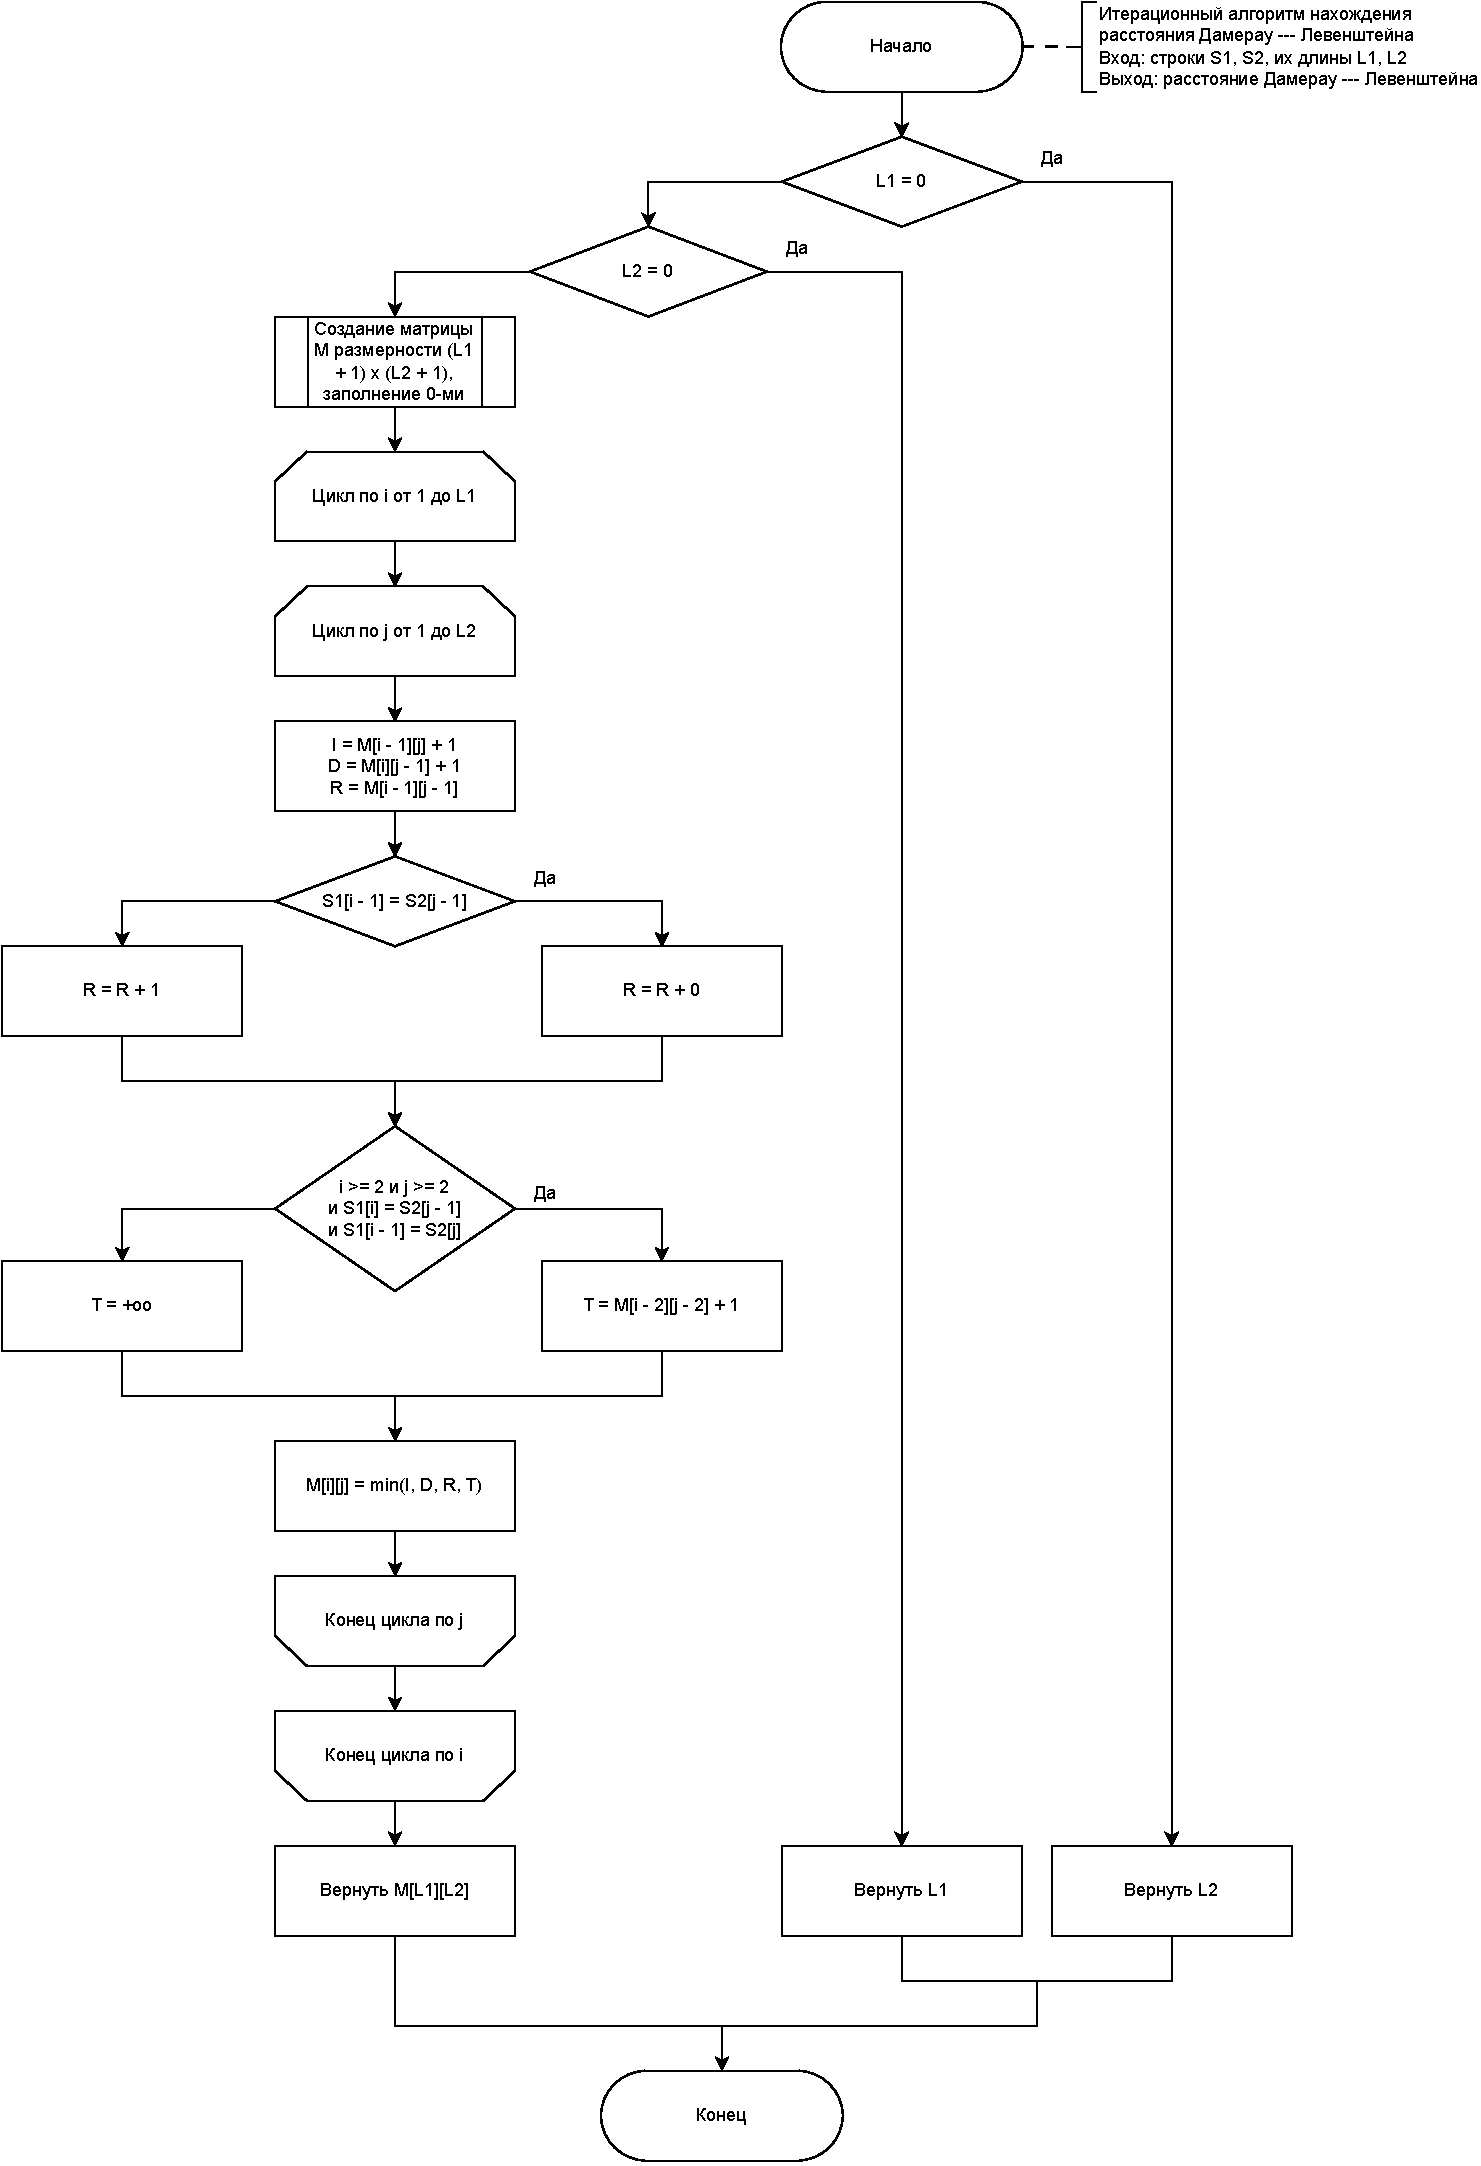
\includegraphics[scale=0.6]{img/dlev_ifm.pdf}
	\caption{Итерационный алгоритм нахождения расстояния Дамерау --- Левенштейна}
	\label{fig:dlifm}
\end{figure}

\begin{figure}[h]
	\centering
	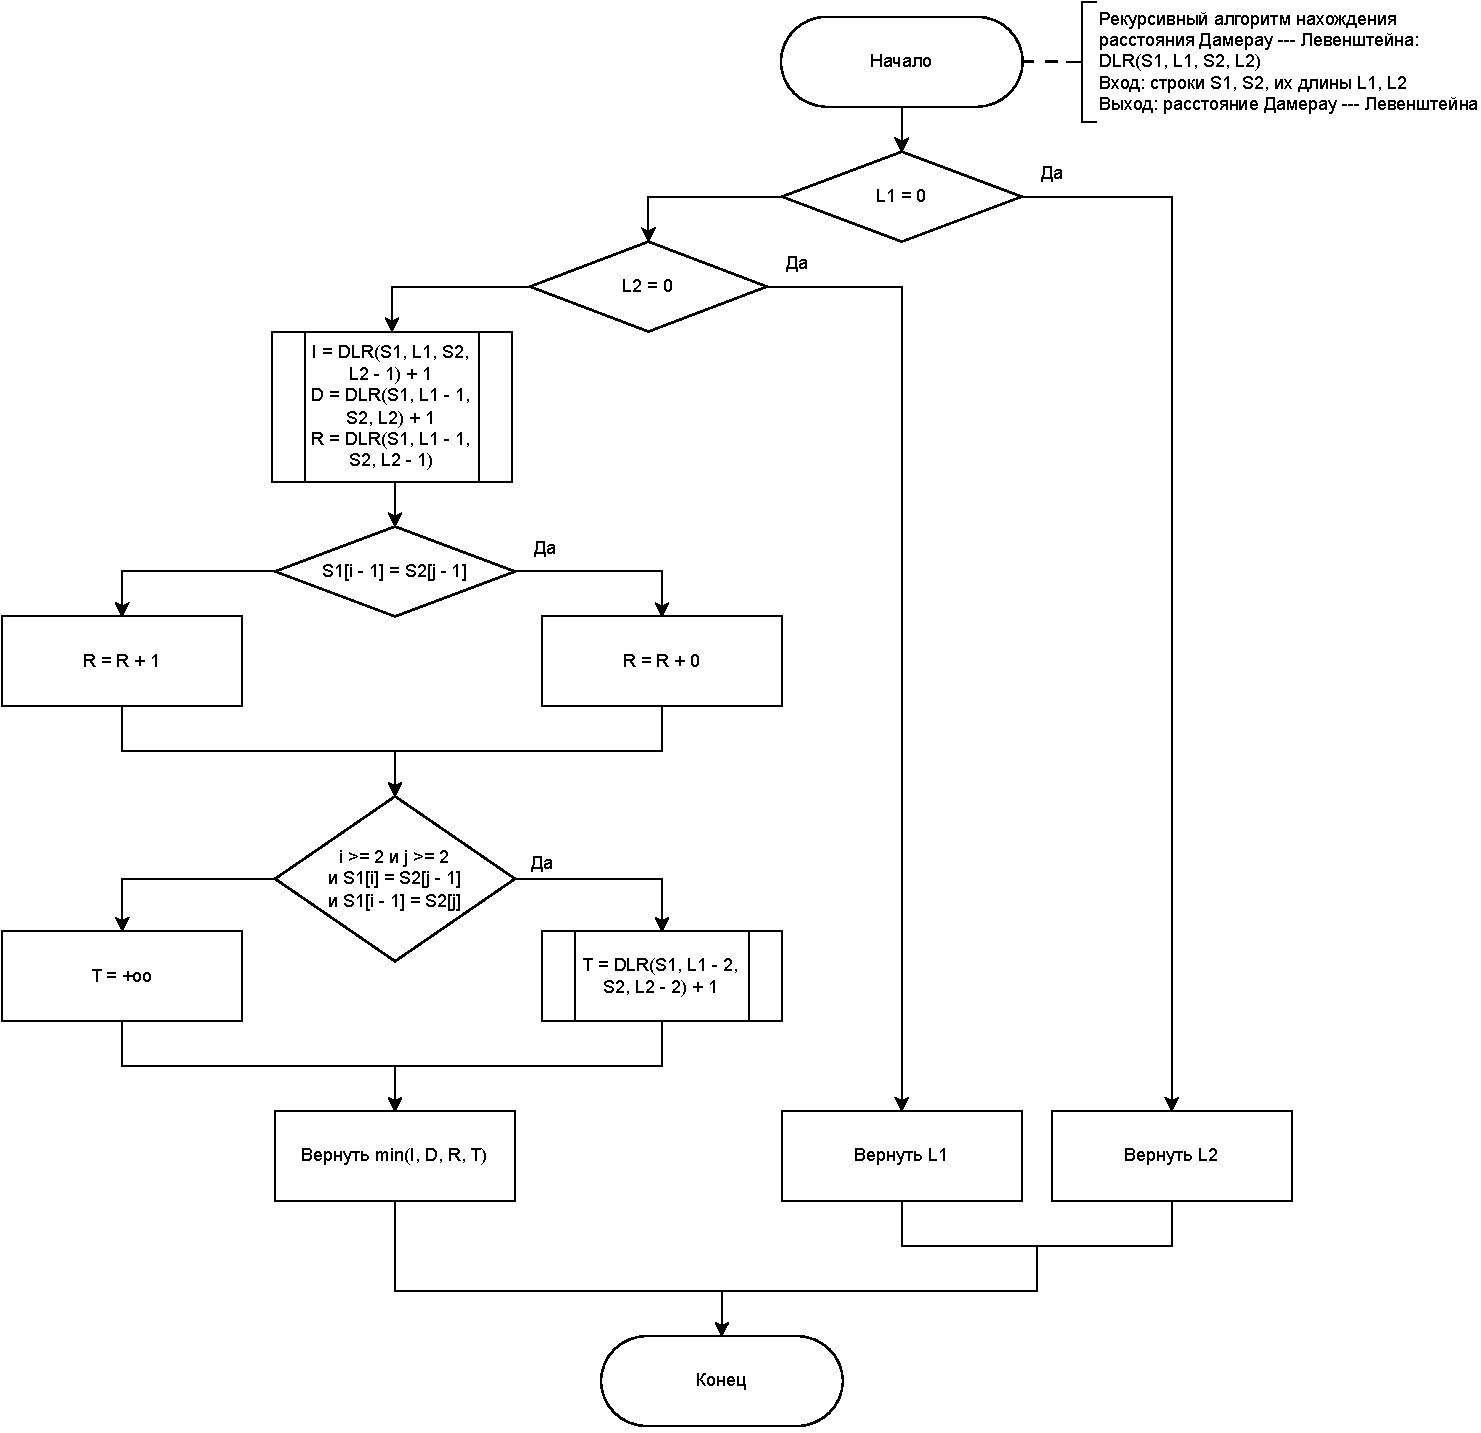
\includegraphics[scale=0.6]{img/dlev_rec.pdf}
	\caption{Рекурсивный алгоритм нахождения расстояния Дамерау --- Левенштейна}
	\label{fig:dlrec}
\end{figure}

\begin{figure}[h]
	\centering
	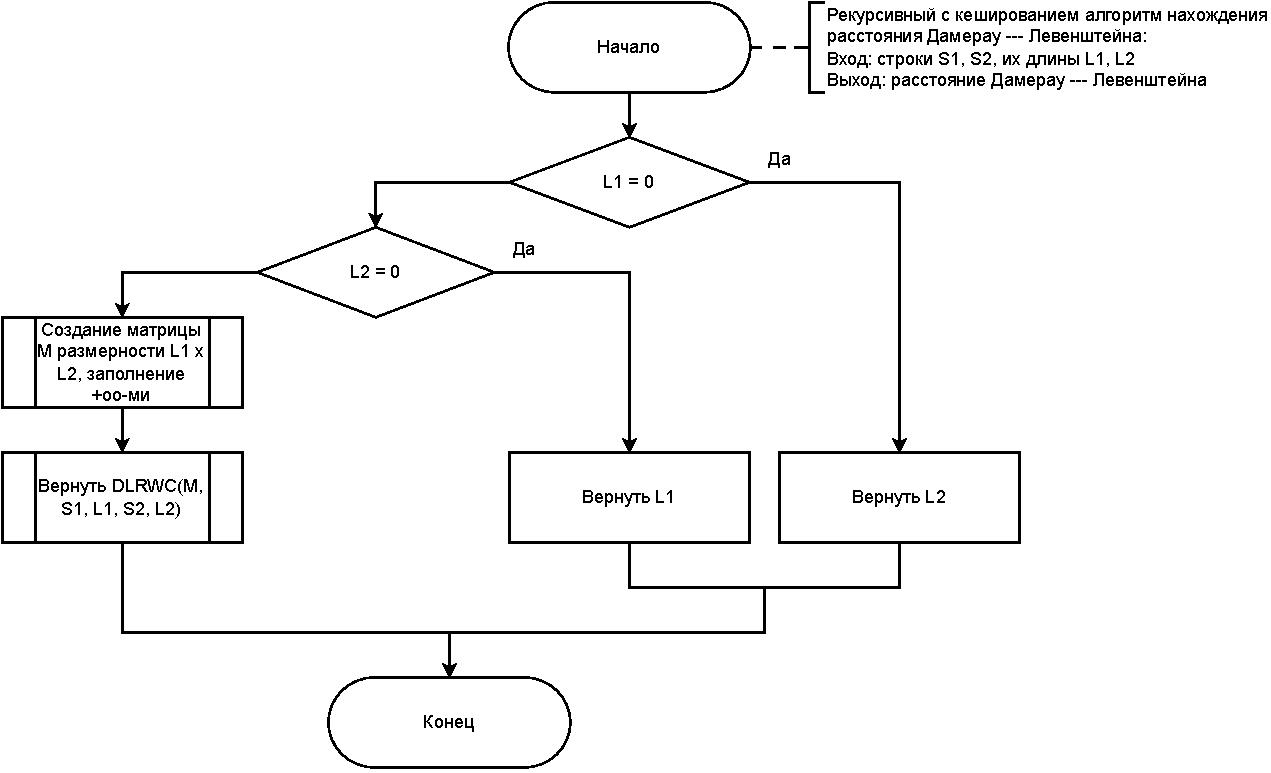
\includegraphics[scale=0.6]{img/dlev_rwc.pdf}
	\caption{Рекурсивный с кешированием алгоритм нахождения расстояния Дамерау --- Левенштейна}
	\label{fig:dlrwc}
\end{figure}

\begin{figure}[h]
	\centering
	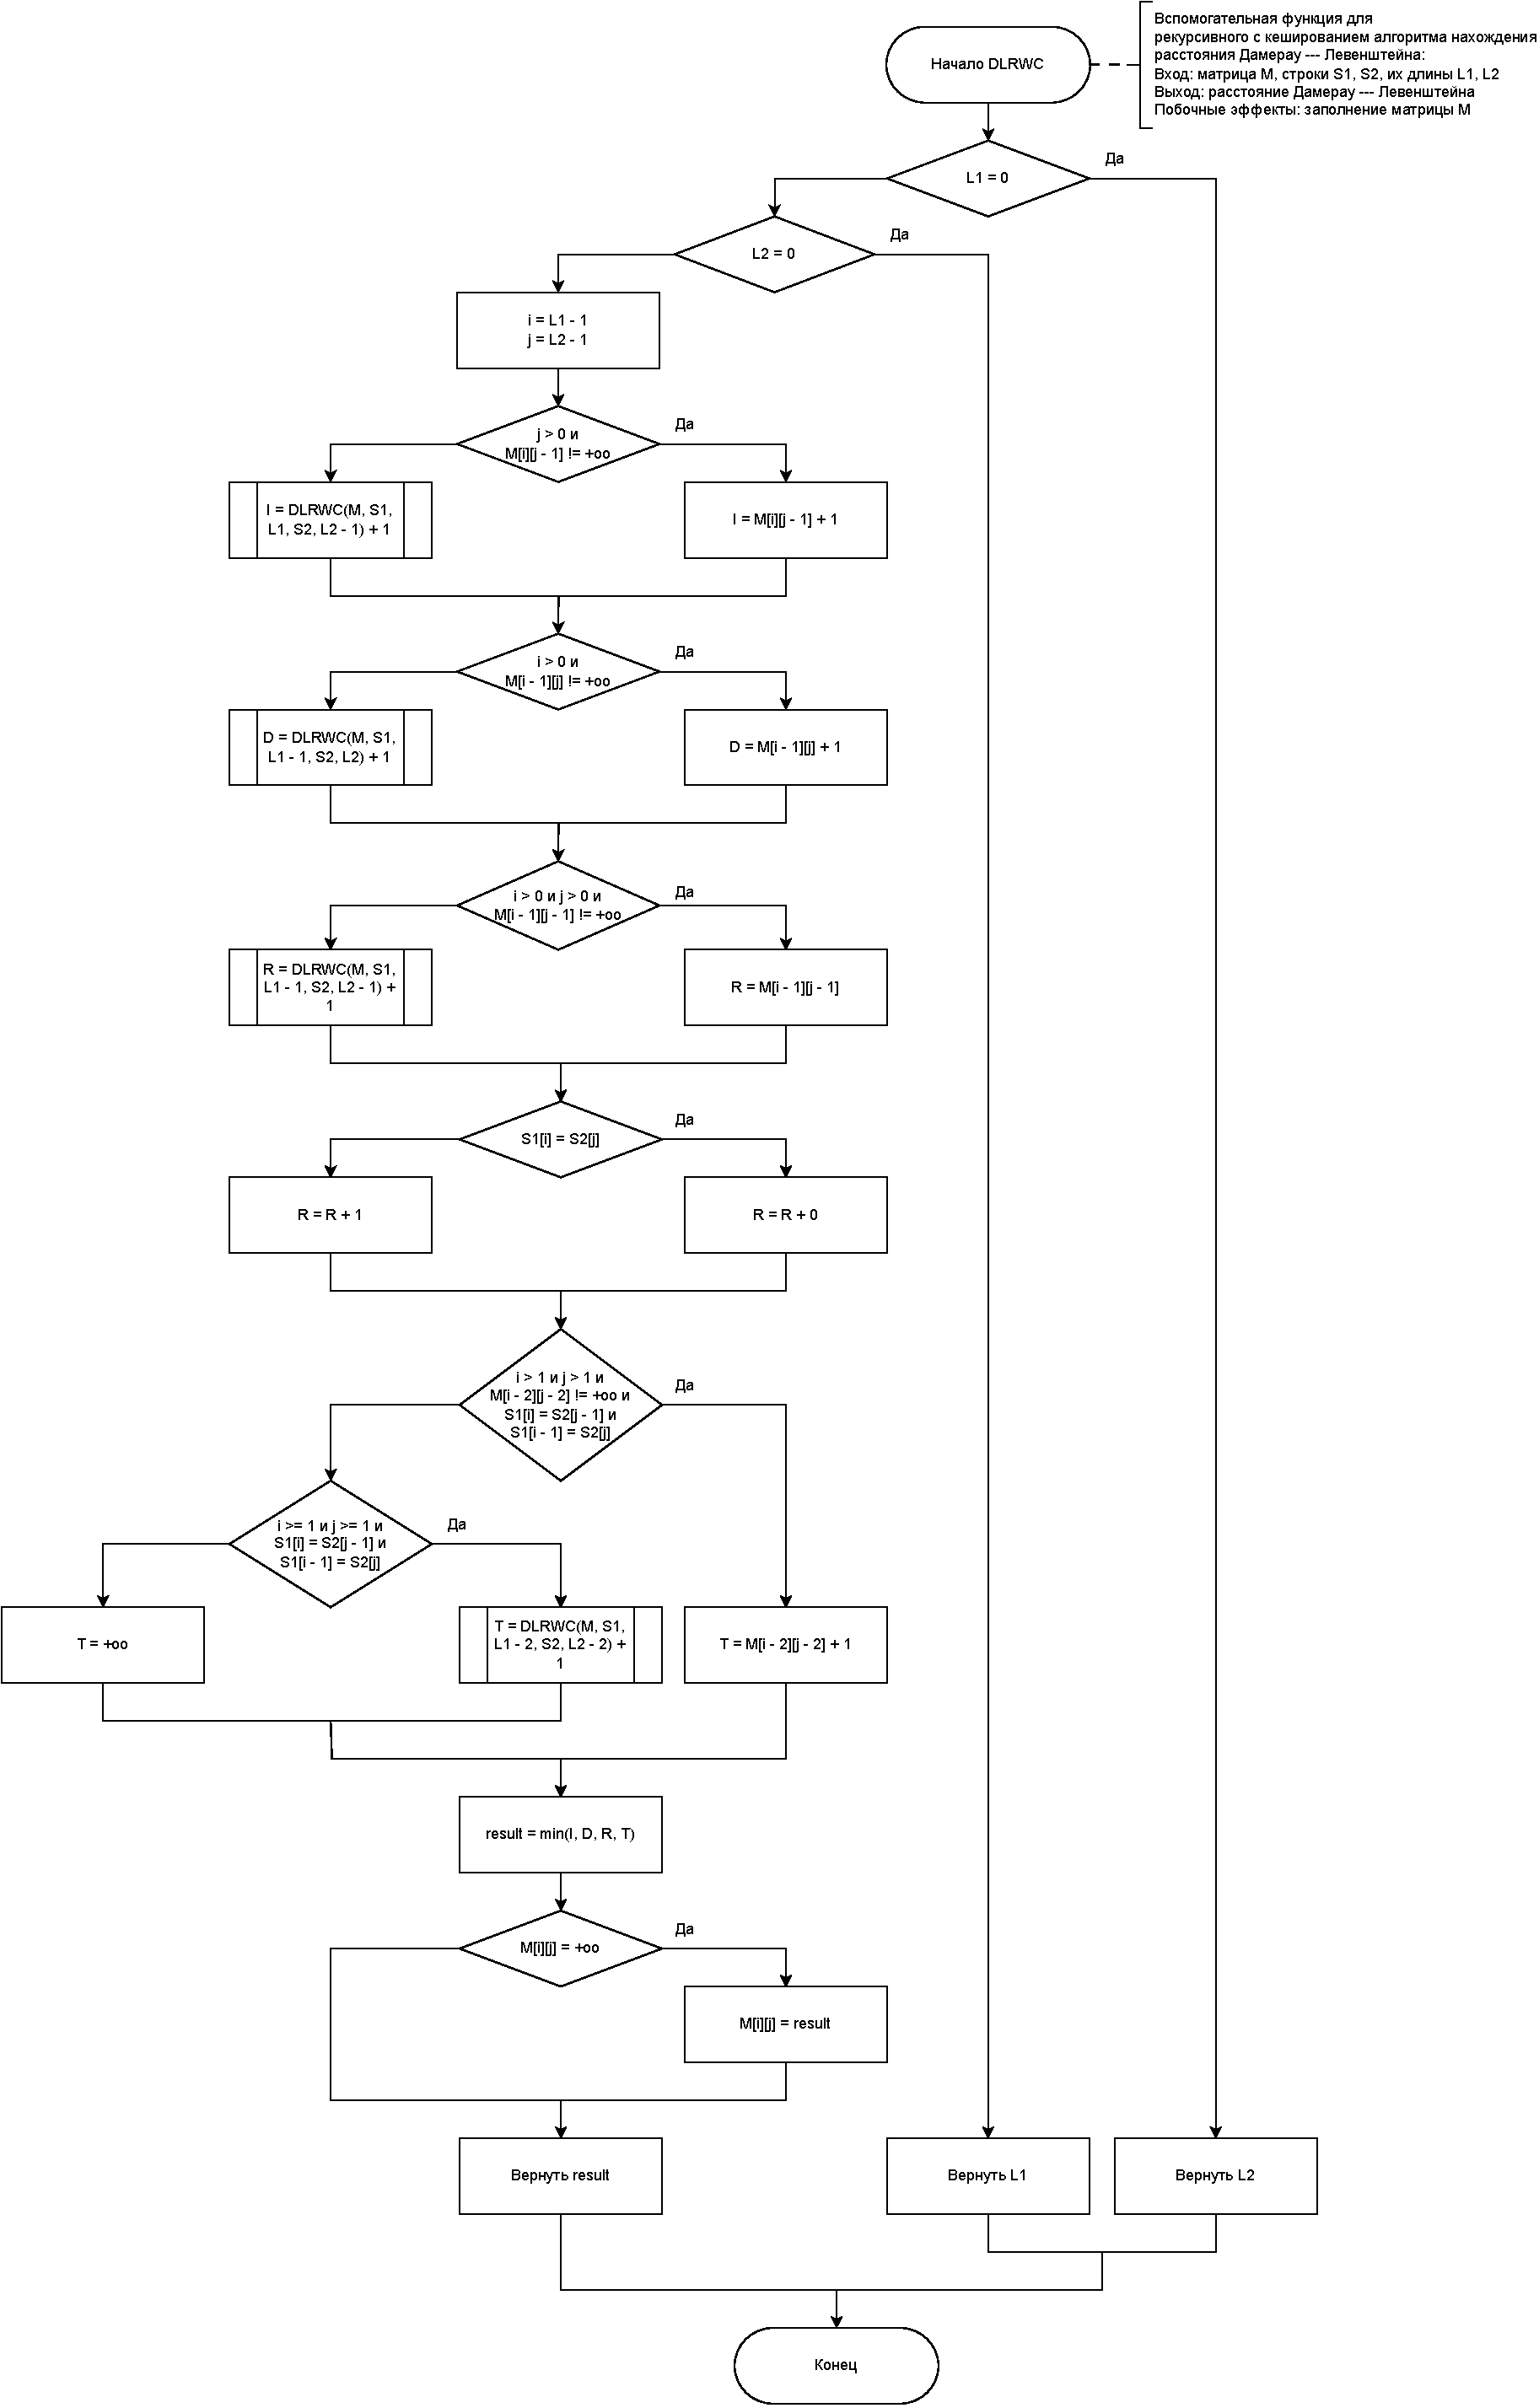
\includegraphics[scale=0.5]{img/dlrwch.pdf}
	\caption{Рекурсивная функция нахождения расстояния Дамерау --- Левенштейна с использованием матрицы в качестве кеша}
	\label{fig:dlrwch}
\end{figure}
